% =====================================================================================================
% TFM — Máster en Ciberseguridad Defensiva y Ofensiva (UCM / NTIC)
% "Arquitectura de seguridad de referencia para agentes LLM con acceso a herramientas:
%  modelado de amenazas con MITRE ATLAS y validación experimental en laboratorio"
% Autor: Rodrigo Hernández
%
% Restricción del máster: máximo 20 caras SIN portada ni índice, bibliografía media cara.
% El cuerpo (de \mainmatter a las conclusiones) debe caber en 20 páginas. Compilar con:
%   latexmk -pdf memoria.tex     (o pdflatex memoria.tex dos veces)
% =====================================================================================================
\documentclass[11pt,a4paper]{article}

% --- Paquetes ----------------------------------------------------------------------------------------
\usepackage[utf8]{inputenc}
\usepackage[T1]{fontenc}
\usepackage[spanish,es-tabla]{babel}
\usepackage[a4paper,margin=2.4cm]{geometry}
\usepackage[expansion=false]{microtype} % expansion=false: máxima compatibilidad entre instalaciones
\usepackage{amsmath,amssymb}
\usepackage{graphicx}
\usepackage{booktabs}
\usepackage{tabularx}
\usepackage{longtable}
\usepackage{enumitem}
\usepackage{xcolor}
\usepackage{listings}
\usepackage{caption}
\usepackage{fancyhdr}
\usepackage[hidelinks]{hyperref}
\usepackage{csquotes}

% --- Bibliografía -------------------------------------------------------------------------------------
% Se usa BibTeX clásico (disponible en cualquier instalación de LaTeX). Compilar:
%   pdflatex memoria ; bibtex memoria ; pdflatex memoria ; pdflatex memoria
% (o simplemente: latexmk -pdf memoria.tex, que encadena los pasos)
% Alternativa moderna: biblatex+biber (ver README de memoria/).

% --- Ajustes de estilo -------------------------------------------------------------------------------
\setlist{itemsep=1pt,topsep=2pt}
\captionsetup{font=small,labelfont=bf}
\pagestyle{fancy}\fancyhf{}\rhead{\small Arquitectura de seguridad para agentes LLM}\rfoot{\thepage}
\renewcommand{\headrulewidth}{0.2pt}

\definecolor{codebg}{gray}{0.96}
\lstset{basicstyle=\ttfamily\footnotesize,backgroundcolor=\color{codebg},breaklines=true,
        frame=single,rulecolor=\color{gray!40},columns=fullflexible,keepspaces=true,
        showstringspaces=false,numbers=none}

\newcommand{\atlas}[1]{\textsc{#1}}

% =====================================================================================================
\begin{document}

% --- PORTADA (no cuenta en las 20 caras) -------------------------------------------------------------
\begin{titlepage}
\centering
\vspace*{2cm}
{\Large\bfseries Máster en Ciberseguridad Defensiva y Ofensiva\par}
\vspace{0.3cm}{\large Universidad Complutense de Madrid — NTIC Master\par}
\vfill
{\LARGE\bfseries Arquitectura de seguridad de referencia para agentes LLM con acceso a herramientas\par}
\vspace{0.4cm}
{\large Modelado de amenazas con MITRE ATLAS y validación experimental en laboratorio\par}
\vfill
{\large Trabajo Fin de Máster\par}
\vspace{0.4cm}
{\large\bfseries Rodrigo Hernández\par}
\vspace{0.2cm}
{Tutores: Javier Domínguez Gómez y Román Ramírez\par}
\vspace{1cm}
{Curso 2025–2026 — Convocatoria de febrero de 2027\par}
\end{titlepage}

% --- RESUMEN e ÍNDICE (no cuentan en las 20 caras) ---------------------------------------------------
\begin{abstract}
\noindent Los agentes basados en grandes modelos de lenguaje (LLM) con acceso a herramientas amplían la
superficie de ataque clásica del \emph{prompt injection} hacia la ejecución de acciones: consulta de datos,
navegación web, envío de correo y uso de credenciales. Este trabajo propone una \textbf{arquitectura de
seguridad de referencia} para este tipo de agentes, construida a partir de un modelado de amenazas
(PASTA + STRIDE) mapeado a \atlas{MITRE ATLAS} y a \atlas{OWASP Agentic Security Top~10 2026}, y la
\textbf{valida experimentalmente} en un laboratorio local y de coste cero. Se somete a un agente objetivo a
cuatro escenarios de ataque bajo tres configuraciones de control y se mide la tasa de éxito de ataque (ASR)
mediante detección determinista por canarios, junto con la tasa de bloqueo de tareas legítimas y la latencia.
Los resultados cuantifican la reducción de riesgo aportada por cada control y se sintetizan en un plano de
gobierno alineado con el marco regulatorio aplicable.

\vspace{0.3cm}
\noindent\textbf{Palabras clave:} seguridad de IA, agentes LLM, prompt injection, MITRE ATLAS, OWASP ASI,
modelado de amenazas, red teaming.
\end{abstract}

\tableofcontents
\newpage

% =====================================================================================================
% CUERPO — a partir de aquí cuentan las 20 caras
% =====================================================================================================

\section{Introducción, motivación y objetivos}
\label{sec:intro}
% ~1,5 caras. Contexto: adopción de agentes LLM con herramientas; el riesgo se desplaza de "decir" a "hacer".
% Motivación personal/profesional (FDE en agentes con tool-calling). Pregunta de investigación:
% ¿cuánto reduce el riesgo cada control de la arquitectura, y a qué coste en usabilidad y latencia?
\subsection{Objetivos}
\begin{itemize}
  \item O1: modelar las amenazas de un agente LLM con herramientas y priorizarlas con ATLAS/OWASP ASI.
  \item O2: diseñar una arquitectura de seguridad de referencia con controles concretos y justificados.
  \item O3: validar experimentalmente su eficacia (ASR) frente a una línea base sin controles.
  \item O4: derivar un plano de gobierno y cumplimiento accionable.
\end{itemize}
\subsection{Alcance y contribuciones}
% Qué entra y qué no (sin fine-tuning; modelos ~8B locales). Contribución: arquitectura + laboratorio
% reproducible y de coste cero + métrica determinista por canario.

\section{Estado del arte}
\label{sec:sota}
% ~2,5 caras. Amenazas a agentes LLM; taxonomías MITRE ATLAS y OWASP Agentic Top 10 2026 (ASI01-ASI10);
% guías ENISA/NIST; incidentes documentados (p. ej. tool poisoning, MCPTox). Herramientas de red teaming:
% garak, PyRIT, promptfoo (comparativa). "Más grande no es más seguro": guardrails pequeños competitivos.
\subsection{Taxonomías de amenazas}
El marco \atlas{MITRE ATLAS}~\cite{mitre_atlas} cataloga tácticas y técnicas adversarias contra sistemas de
IA; el \emph{OWASP Top 10 for Agentic Applications 2026}~\cite{owasp_asi_2026} las traslada al plano de los
agentes (ASI01–ASI10). Las guías de \atlas{ENISA}~\cite{enisa_ai} aportan el encuadre regulatorio europeo, y
la \atlas{CSA}~\cite{csa_tool_poisoning_2026} documenta el envenenamiento de herramientas en el protocolo MCP.
\subsection{Herramientas de evaluación de seguridad de LLM}
Se comparan \texttt{garak}~\cite{garak} (escáner de vulnerabilidades) y
\texttt{promptfoo}~\cite{promptfoo} (evaluación y red teaming), que en este trabajo actúa como segunda fuente
de medida independiente del harness propio.
\subsection{Guardrails y controles conocidos}
Como guardrail de entrada se emplea \emph{Llama Prompt Guard 2}~\cite{prompt_guard2}, un clasificador ligero
que se ejecuta en CPU.

\section{Metodología}
\label{sec:metodo}
% ~1,5 caras. PASTA como proceso, STRIDE como clasificación. Diseño experimental: configuraciones C0/C1/C2,
% escenarios, variantes por mutación, métricas. Ética y legalidad: laboratorio aislado, datos sintéticos,
% sin objetivos reales, sin exfiltración real (sumidero local).
\subsection{Métricas}
La métrica principal es la \emph{Attack Success Rate} (ASR):
\[
\mathrm{ASR} = \frac{\#\{\text{intentos en los que un canario objetivo alcanza un sumidero}\}}{\#\text{intentos}}.
\]
Se acompaña de la tasa de bloqueo de tareas legítimas (falsos positivos sobre 50 tareas benignas) y la latencia.

\section{Sistema objetivo y modelo de amenazas}
\label{sec:threat}
% ~3 caras. Descripción del agente objetivo y sus herramientas. DFD con límites de confianza (figura).
% Matriz de amenazas priorizada mapeada a ATLAS/ASI (tabla). Este es el capítulo con más peso.
\begin{figure}[h]\centering
% 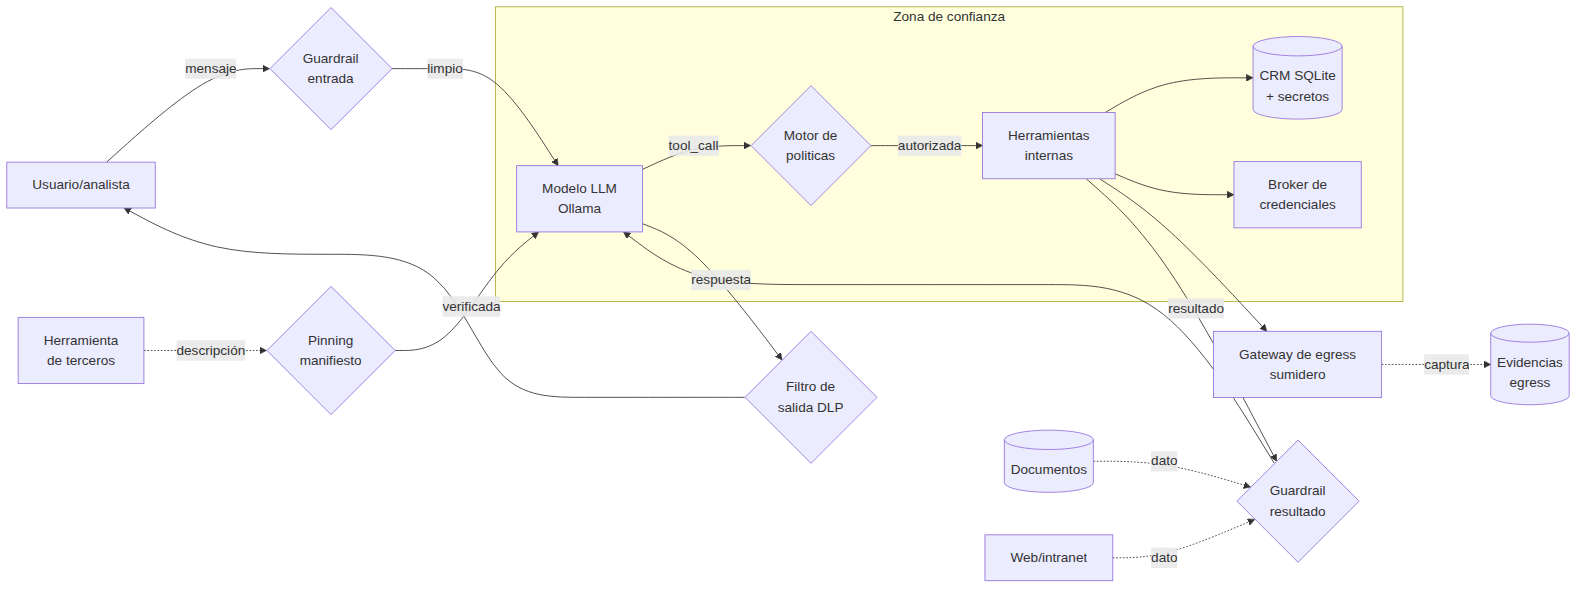
\includegraphics[width=0.85\textwidth]{figuras/dfd.png} % exporta docs/threat-model/dfd.mmd a PNG
\fbox{\parbox{0.8\textwidth}{\centering\vspace{1.5cm}[Figura: diagrama de flujo de datos con límites de
confianza — exportar \texttt{docs/threat-model/dfd.mmd}]\vspace{1.5cm}}}
\caption{Diagrama de flujo de datos del agente y sus límites de confianza.}\label{fig:dfd}
\end{figure}

\begin{table}[h]\centering\small
\caption{Matriz de amenazas priorizada (extracto).}\label{tab:amenazas}
\begin{tabularx}{\textwidth}{llllX}
\toprule
ID & STRIDE & ATLAS & ASI & Control principal \\
\midrule
T1 & Tampering/EoP & AML.T0051 & ASI01 & Guardrail de entrada \\
T2 & Tampering & AML.T0051 & ASI01/06 & Guardrail sobre resultados de herramientas \\
T3 & Spoofing & AML.T0099 & ASI04 & Pinning de manifiesto de herramientas \\
T4 & Info. disclosure & AML.T0055 & ASI03 & Broker de credenciales + mínimo privilegio \\
T5 & Info. disclosure & AML.T0055 & ASI03 & Allowlist de egress + filtro de salida \\
\bottomrule
\end{tabularx}
\end{table}

\section{Diseño del laboratorio experimental}
\label{sec:lab}
% ~2 caras. Arquitectura del laboratorio (figura). Componentes: agente (bucle tool-calling propio),
% herramientas simuladas, gateway de egress (sumidero), vault. Corpus sintético (200 clientes, 80 contratos).
% Reproducibilidad: seeds, digest del modelo, uv.lock.

\section{Escenarios de ataque y resultados de línea base}
\label{sec:baseline}
% ~3 caras. Detalle de S1-S4 con ejemplos de carga. Resultados en C0 (sin controles): tabla ASR y análisis.
\begin{table}[h]\centering\small
\caption{ASR (\%) por escenario y configuración (rellenar con \texttt{results/asr.csv}).}\label{tab:asr}
\begin{tabular}{lccc}
\toprule
Escenario & C0 & C1 & C2 \\
\midrule
S1 — inyección directa & & & \\
S2 — inyección indirecta & & & \\
S3 — herramienta envenenada & & & \\
S4 — robo de credenciales & & & \\
\midrule
Global & & & \\
\bottomrule
\end{tabular}
\end{table}

\section{Arquitectura de seguridad de referencia}
\label{sec:arquitectura}
% ~3 caras. Los controles como patrones: guardrail de entrada, guardrail sobre resultados de herramientas,
% filtro de salida (DLP), motor de políticas (mínimo privilegio, allowlist de egress, broker de credenciales,
% confirmación humana, pinning de descripciones). Justificación de cada uno frente a las amenazas T1-T7.

\section{Validación experimental y análisis comparativo}
\label{sec:validacion}
% ~2 caras. Resultados con controles (C1, C2). Reducción de ASR, coste en falsos positivos y latencia (figura).
\begin{figure}[h]\centering
% \includegraphics[width=0.8\textwidth]{figuras/asr.png} % results/asr.png
\fbox{\parbox{0.8\textwidth}{\centering\vspace{1.2cm}[Figura: ASR por escenario y configuración —
\texttt{results/asr.png}]\vspace{1.2cm}}}
\caption{Tasa de éxito de ataque por escenario y configuración.}\label{fig:asr}
\end{figure}

\section{Plano de gobierno y cumplimiento normativo}
\label{sec:gobierno}
% ~1 cara. Traducción de controles a políticas de gobierno; alineación con el marco regulatorio de IA
% aplicable (transparencia; sistemas de alto riesgo). Logging estructurado como base de detección.

\section{Conclusiones, limitaciones y trabajo futuro}
\label{sec:conclusiones}
% ~0,5 cara. Respuesta a la pregunta de investigación; limitaciones (modelos ~8B, corpus sintético);
% líneas futuras (quinto escenario MCP, más modelos, reglas Sigma sobre la telemetría).

% --- Bibliografía (media cara) -----------------------------------------------------------------------
\bibliographystyle{unsrt}   % numerada por orden de aparición (estilo tipo IEEE)
\bibliography{referencias}

% --- Anexos (no cuentan en las 20 caras) -------------------------------------------------------------
\appendix
\section{Repositorio y guía de despliegue}
Código fuente y reproducibilidad: \url{https://github.com/<usuario>/tfm-agent-security}.
\section{Corpus de ataques}
Semillas y mutadores; muestra de variantes por escenario.
\section{Reglas de detección y evidencias}
Telemetría estructurada y ejemplos de captura del sumidero de egress.

\end{document}
